\section{Scattering}

The use of scattering techniques to probe soft condensed matter systems is commonplace. In this work, we have focussed on the use of small angle scattering (SAS), reflectometry, and grazing incidence small angle scattering (GiSAS) techniques. These are particularly appropriate for application to soft condensed matter systems due to the length scales capable of being probed being similar to the persistence length of the soft condensed matter systems. The length scales covered for such techniques is from around \SI{1}{\nano\metre} to \SI{100}{\nano\metre}, as is shown in Figure \ref{fig:lengths}. Since it is the equilibrium structures(s) under study, there is no interest in the system dynamics. Therefore, the system can be studied using exclusively elastic scattering techniques, where there is no energy transfer between the probing radiation and the system. This is in contrast to inelastic scattering where energy transfer occurs; facilitating the measurement of system dynamics, such as the dynamical modes of polymers of lipid bilayers.\cite{Sakai2009, Farago2009} The techniques mentioned above all involve the use of elastic scattering and therefore probe the system equilibrium structure.
%
\begin{figure}
	\centering
	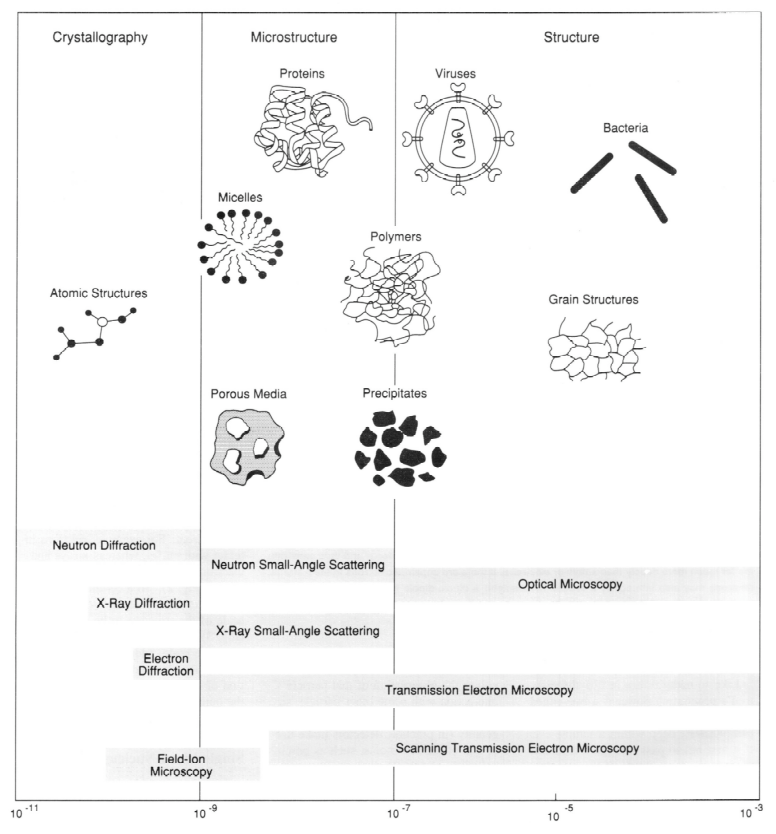
\includegraphics[width=0.7\textwidth]{theory/length}
	\caption{A representation of how different techniques can be used to probe various length scales, from Ref \cite{Sivia2011}.}
	\label{fig:lengths}
\end{figure}
%

Both X-ray and neutron scattering techniques are discussed and used in this work. From an experimental viewpoint, there are significant differences between an X-ray scattering and a neutron scattering experiment. However, there is little variation in terms of the data analysis, where the differences are limited to; the nature of the scattering lengths, and the higher background that is present in the neutron scattering experiments.

\subsection{The scattering vector}

The scattering of some probing radiation, by some sample can be represented as shown in Figure \ref{fig:scat}. Since only elastic scattering is being considered, there will be no change in the frequency of the radiation, $\omega_i = \omega_f$. This means that only the wavevector, $\mathbf{k}$, can change, $\mathbf{k}_i\neq \mathbf{k}_f$. The difference between the incident and final wavevectors is the scattering vector, $\mathbf{q}$, where,
%
\begin{equation}
	\mathbf{q} = \mathbf{k}_i - \mathbf{k}_f.
\end{equation}
%
%
\begin{figure}
	\centering
	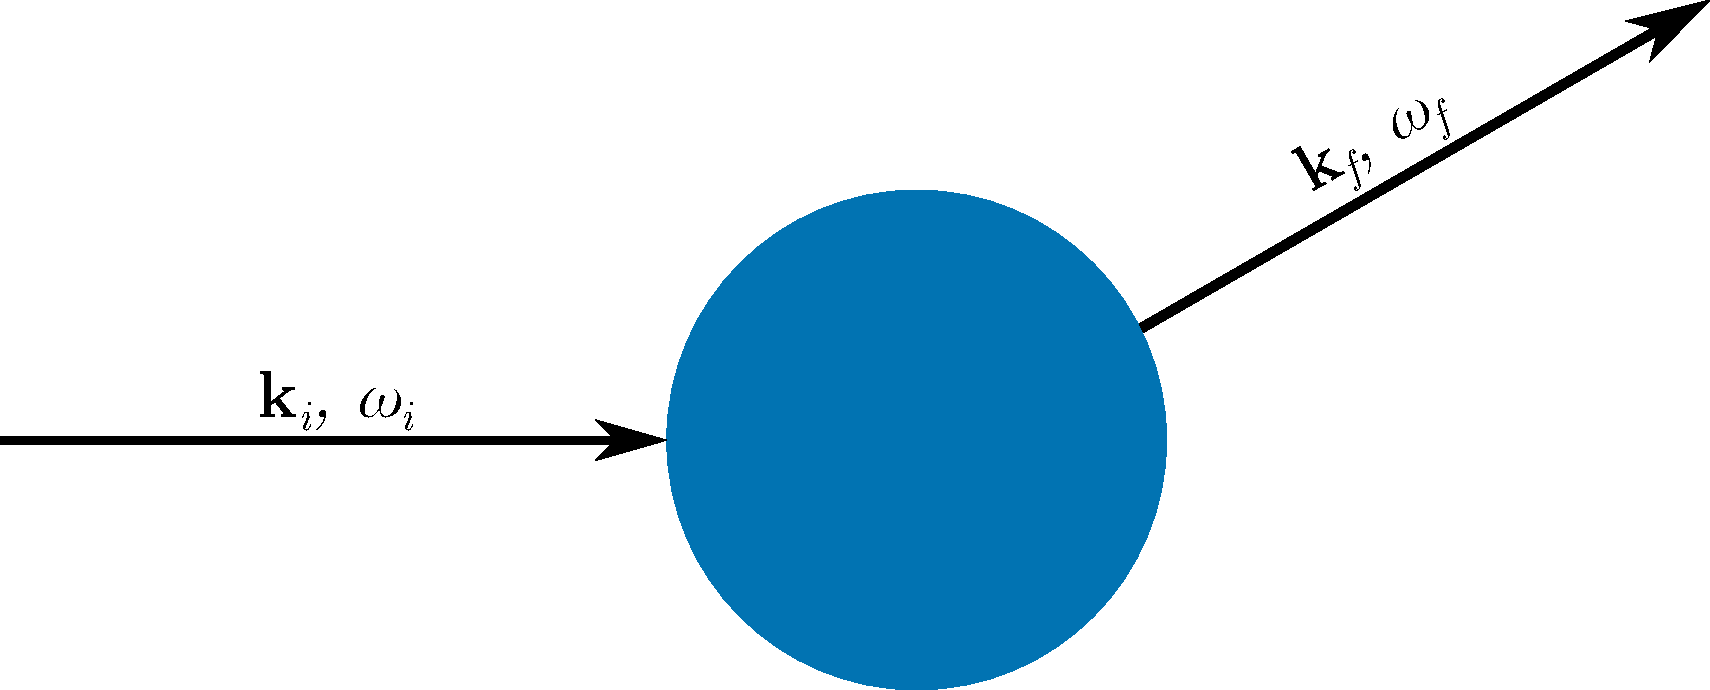
\includegraphics[width=0.7\textwidth]{theory/scat}
	\caption{A schematic of the scattering of some probing radiation by a sample (blue circle), adapted from Ref \cite{Sivia2011}.}
	\label{fig:scat}
\end{figure}
%
The scattering vector strictly has units of \si{\per\meter}, however it is often more practical to use \si{\per\nano\meter} or \si{\per\angstrom}. Throughout this work, units of reciprocal \AA ngstrom will be wherever possible. Since the frequency of the probing radiation does not change during an elastic scattering event, the wavelength, $\lambda$, will also not change, meaning that the moduli of the incident and final wavevectors are,
%
\begin{equation}
	|\mathbf{k}_i| = |\mathbf{k}_f|=\frac{2\pi}{\lambda}.
	\label{equ:wavevec}
\end{equation}
%
This means that only the angle will change during the elastic scattering event. The vector diagram in Figure \ref{fig:scatvec} can be used to describe the geometry of an elastic scattering event. From this, and Equation \ref{equ:wavevec}, the value of $q$, where $q = |\mathbf{q}|$ can be shown as,
%
\begin{equation}
	q = \frac{4\pi\sin{\theta}}{\lambda}.
\end{equation}
%
\begin{figure}
	\centering
	\includegraphics[width=0.7\textwidth]{theory/scatvec}
	\caption{A vector diagram describing an elastic scattering event, adapted from Ref \cite{Sivia2011}.}
	\label{fig:scatvec}
\end{figure}
%
However, this fails to fully capture the three dimensional nature of the scattering event. Hence, it is necessary to describe the scattering with spherical coordinates, $2\theta$, and $\phi$, such that the incoming and outgoing radiation can be described as,
%
\begin{equation}
	\begin{aligned}
		\mathbf{k}_i & = \bigg(0, 0, \frac{2\pi}{\lambda}\bigg), \\
		\mathbf{k}_f & = \frac{2\pi}{\lambda}(\sin{2\theta}\cos{\phi}, \sin{2\theta}\sin{\phi}, \cos{2\theta}),
	\end{aligned}
\end{equation}
%
where, $|\mathbf{k}_f| = \sfrac{2\pi}{\lambda}$. This allows the scattering vector to be written,
%
\begin{equation}
	\mathbf{q} = \frac{4\pi\sin{\theta}}{\lambda}(-\cos{\theta}\cos{\phi}, -\cos{\theta}\sin{\phi},\sin{\theta}).
\end{equation}
%
For an isotropic scattering pattern, it is the magnitude of the scattering vector, $q$, that is measured. In partical terms, the scattering vector allows for easy comparison of measurements made at different radiation wavelengths.
